\documentclass[11pt]{article}

\usepackage[style=apa,sortcites=true,sorting=nyt,backend=biber]{biblatex}
\usepackage{graphicx}
\usepackage{booktabs}
\DeclareLanguageMapping{american}{american-apa}
\addbibresource{bibliography.bib}

\title{ BabyLM Challenge Report }
\author{ Jelle Roeloffs }
\date{\today}

\begin{document}
\maketitle

\section{Project goal}

\paragraph{}
Almost a year ago, \textcite{jiang2023zip} published a paper detailing a novel parameter-free technique for text classification. Their theory was that the Kolmogorov complexity of two texts combined (as approximated with gzip) reveals information about the text that allows for classification that is more accurate than other similar ``dumb'' methods like Bag-of-Words or TF.IDF, despite the technique sounding similar in theory.

\paragraph{}
Their technique is to calculate the so-called \textit{ncd}, or Normalised Compressed Distance, to then use a K-nearest-neighbour classifier with the \textit{ncd} as the distances between the texts. This \textit{ncd} is calculated as follows, where $C(x)$ is the size of $x$ after being compressed with gzip:
$$ NCD(y, y) = \frac{C(xy) - \min(C(x),C(y))}{\max(C(x), C(y))} $$

\paragraph{}
In their abstract, they claim their technique is competitive with non-pretrained deep learning methods, and say it outperforms BERT in all their tried cases, which likely is why it has received somewhat widespread popular attention. The details of their results are more nuanced, however. They calculated their system to have given a correct response if either of the two most likely classes the model put out was correct, which gave it quite the advantage. Their argument for this was that it would simulate how the model would perform with optimal parameter selection, however, attempts to replicate the results with fair assessment techniques have so far failed with all parameter sets, with it performing similarly to Bag-of-Words \parencite{opitz2023gzip}.

\paragraph{}
Despite this, their techniques are interesting in many ways. It has long been argued that good language modelling \textit{is} language compression \parencite{deletang2023language}, where most transformer models are able to perform high-quality lossless text compression when wired to loop back on themselves.

\paragraph{}
With all this in mind, I thought it would be interesting to try to use these zip-based techniques on other problems, not because they \textit{should} would, but because they \textit{might}. Specifically, it would be most interesting to use these techniques on tasks with little training data available, to then compare it to other techniques using the same training set, as these zip-based techniques are said to comparatively work better with little data.

For this assignment, the task was to play around with the BabyLM challenge, which is the challenge to train a language model on a relatively small data set, which seemed like the perfect opportunity to fool around with some zip models.


\subsection{Dataset Description}
\paragraph{}
The main subject of the BabyLM challenge is its training data. The ``Baby'' in ``BabyLM'' refers to it. The data is an attempt at capturing the language input a 13-year-old child would have had in their lifetime. There are two tracks: one with ten million words, and another with one hundred million words (As well as a multi-modal track that I completely ignored,) These respectively are the lower and upper bound of the amount of language input a 13-year-old would have had. For this project, I only used the ten million words set, mostly because the models were taking up more than enough computation time like that already.

\paragraph{}
The data distributed for BabyLM consists of six parts, all of which are selections of data from in-distribution data sets: \verb|bnc_spoken|, \verb|childes|, \verb|gutenberg|, \verb|open_subtitles|, \verb|simple_wiki|, and \verb|switchboard|.

\paragraph{}
Some basic information about these can be found in the table below. Here, the ``naive'' way to split sentences is with linebreaks (which roughly equate to sentences in the input), and the naive way to count words is to split on whitespace. The proper tokens and sentences are instead done with \verb|nltk|, making use of the default \verb|nltk.word_tokenize()| and \verb|nltk.sent_tokenize()| \parencite{loper2002nltk} (The script that retrieves this data can be executed as \verb|python -m zip_lm.scripts.get_data_metrics|)

\paragraph{}
\resizebox{1 \textwidth}{!}{
\begin{tabular}{lrrrrrrr}
\toprule
index & bnc spoken & childes & gutenberg & subtitiles & simple wiki & switchboard & combined \\
\midrule
nr words naive & 926424 & 2082717 & 2524804 & 1989283 & 1344535 & 128706 & 9414580 \\
nr unique words & 926424 & 2082717 & 2524804 & 1989283 & 1344535 & 128706 & 9414580 \\
mean word length & 4.04 & 3.77 & 4.23 & 4.02 & 4.77 & 3.86 & 4.23 \\
nr sentences naive & 90000 & 537662 & 62155 & 360000 & 40432 & 18000 & 1058681 \\
mean words per sentence & 10.29 & 3.87 & 40.62 & 5.53 & 33.25 & 7.15 & 8.89 \\
\midrule
nr words nltk & 1095877 & 2877371 & 3075473 & 2655822 & 1593357 & 166698 & 11962078 \\
nr unique tokens nltk & 24556 & 24189 & 59873 & 61648 & 84457 & 6804 & 164319 \\
nr sentences nltk & 90052 & 538370 & 152248 & 362106 & 98633 & 18386 & 1268376 \\
mean tokens per sentence & 12.17 & 5.34 & 20.20 & 7.33 & 16.15 & 9.07 & 9.43 \\
\bottomrule
\end{tabular}
}

\paragraph{}
As is expected from the goal of this data, the \verb|childes| dataset has a lower mean word length and a lower amount of words per sentence. Moreover, the \verb|simple_wiki| and \verb|gutenberg| datasets have the highest mean word length and amount of words per sentence, which is also expected, as these are datasets of written language (instead of transcribed spoken language), which is generally more semantically and syntactically complex.

\paragraph{}
The ten most common parts of speech were also extracted, but nothing interesting could be concluded from them, they are generally the most common PoS in the English language, with slight variations that can be explained through the variation of sentence length (like the \verb|childes| having more end of sentence tokens.) These can be found in the result data distributed with this report.


\paragraph{}
The data can also be observed to follow Zipf's law \parencite{zipf2013psycho, zipf2016human}, specifically comparing against the adaptation of \textcite{mandelbrot1953informational}.
\begin{figure}[ht]
    \centering
    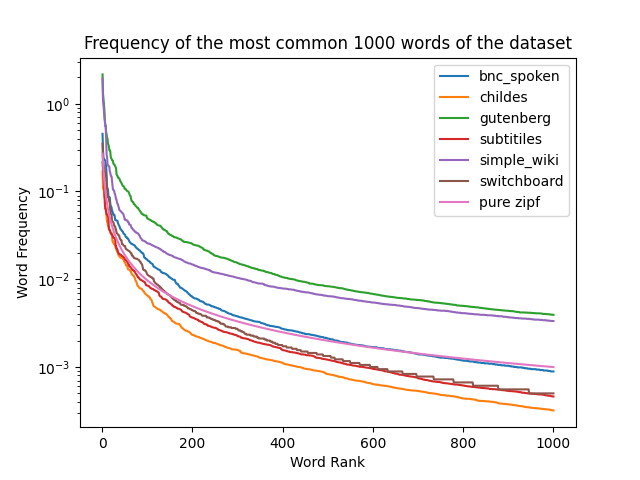
\includegraphics[width=\textwidth]{figures/zipf.png}
    \label{fig:zipf}
\end{figure}

\paragraph{}
Finally, a rudimentary word frequency analysis was performed, comparing the datasets with each other as well as with the Brown corpus \parencite{francis1979brown}, where the only interesting spikes to observe are from pronouns. \verb|bnc_soken|, \verb|subtitiles|, and \verb|switchboard| all have disproportionally many instances of ``he'' and ``his'' when compared to the brown corpus. This might suggest a higher male-first bias in these texts than is the case of English language data generally.


\subsection{The gzip approach}

\paragraph{}
For my new gzip language model, I wanted to try to adapt this \verb|ncd| score to instead return the log-likelihood of a piece of text (which is what a language model \textit{is}). Many techniques might work for this in theory, but many of them fail because of their high computational needs. (calculating the \verb|ndc| of every sentence to every sentence for the 10M track, still is $10,000,000^2$ compressions, which would take years to compute even on the most modern CPUs)

\paragraph{}
The most trivial viable implementation of a \verb|ncd|-based language model would be to use
$$P(x) = softmax(f\{ncd(x, y) | y \in \mathrm{Dataset}\})$$
where $f()$ would be some function to aggravate the softmaxes, like the mean or some quotient. In theory, this computation would still require the $10,000,000^2$ compressions, however, most of that computation is equal between calculations of the log-likelihood, meaning it can be factored out as a constant, which, with how I will use the BLiMP evaluation method later, means we can ignore (or approximate) it for this experiment.

\paragraph{}
Another method (that is again only permitted because of how we will do evaluation later), is to use a bootstrap test \parencite{hesterberg2011bootstrap}, which is a statistical trick that comes from computational econometrics. This test would not compute the log-likelihood of a sentence but instead calculate the chance that a given sentence would be a part of the training set, given some similarity metric (in this case, the \verb|ncd| and some $T$, which is again an aggravation function.) Of course, it is possible to turn this chance into an actual log-likelihood by making use of the softmax function but is not needed for this paper.

\paragraph{}
Both of these methods had to be heavily optimized to allow them to be trained on ten million word data sets, but could ultimately be implemented to spend less than a minute training and a little over fifteen seconds inferring a single input (the latter being the limiting factor for the following experiments). The exact methods that were used (as well as any other implementation details) can be found at \verb|src/zipmodels.rs|


\subsection{Baselines}

\paragraph{}
The zip models were compared to several baseline models. Of course, one of these baselines is guessing randomly, but the others should get their introduction.

\subsubsection{The N-gram baseline}

\paragraph{}
Being a simple calculation of the definition of a language model, of log-likelihood, n-grams are a good baseline. Because of data sparsity, a high N usually cannot be chosen, and, for this experiment, $N=1$ (which is to say, accumulated word frequencies) and $N=2$ were used as benchmarks.

For a proper test, one might have wanted to use the n-gram model from nltk \parencite{loper2002nltk} or kenlm \parencite{heafield2011kenlm}, but, as this benchmark is also one that served as a programming template, a custom model was programmed, which used a quite naive tokenizer, and did not have a way to deal with out-of-vocabulary input (simply returning a chance of 0). Arguably, this hurts the present experiment \textit{as an experiment}, but benefits the present paper \textit{as an assignment}.

\subsubsection{The T5 Baseline}

\paragraph{}
T5 \parencite{raffel2020exploring} is a language model developed by a research team at Google, which, though not the state of the art in the world of transformers and deep neural networks, is one of the large names in that space. The primary innovation of this model is the now-commonplace idea to turn all tasks into a text-to-text format. Ideally, a version of T5 with a small number of parameters would be custom-trained on the provided data set as a benchmark. However, there were no computational resources available to do this \footnote{Tough I do provide a script to do this, to show I know how to, as that was part of the points}. Instead, a pre-trained version of T5-base, which is a version of the model with 220 million parameters (over the 11 billion of the full model), was downloaded from huggingface and used as a benchmark model.

\section{Evaulation}

\paragraph{}
For model evaluation, a subset of the evaluation of the original BabyLM challenge is used. Only a subset was used for two reasons. First and foremost, the zip models took a rather long time per inference, meaning even this subset took a full day of compute. Secondly, certain other training sets (such as (Super)GLUE), were not easily implementable in terms of pure log-likelihood.

A more complete paper might have also used a data set like CoLA \parencite{warstadt2019cola}, which would have been easy to add on a technical level, or other also applicable benchmarks, but this was not done because of running time constraints.

\subsection{Evaulation Methods used: BLiMP}
\paragraph{}
The only evaluation method that was used from the BabyLM challenge is BLiMP (Benchmark of Linguistic Minimal Pairs) \parencite{warstadt2020blimp}

\paragraph{}
BLiMP is a training set for grammatical acceptability. One of the problems of testing language models is that it is very hard to evaluate \textit{what} it is that a model is learning, by providing minimal pairs (things that only differ a minimal amount whilst still creating a different outcome, in this case, grammatical/ungrammatical), BLiMP makes it a lot harder for a model to ``cheat'' its way through a test, meaning one can be more certain that a model has indeed captured the information it was meant to capture.

\paragraph{}
In many ways, it can be argued Blimp is \textit{too good} a test set for a simple model like this. Other naive methods, such as bag-of-words and n-grams, are known to not perform better than random on this set, which makes it hard to distinguish between them. However, if the claims of \textcite{jiang2023zip} ring true and these zip models outperform BERT, they could still perform better than random on this test set.

\subsubsection{Description of the \textit{phenomena} BLiMP covers}
\paragraph{}
The BLiMP test set is separated into twelve \textit{phenomena}, each containing a handful of \textit{paradigms}. The paradigms will be discussed here in short:
\begin{itemize}
\item[] \textsc{Anaphor Agreement}: Anaphora (Also known as reflexive pronouns, e.g. \textit{herself} or \textit{themself}) must be congruent (which, in English, means to agree in person, number, gender and animacy) with their antecedent (who or what they are referring to).
    \begin{itemize}
        \item[1a)] The Machine has destroyed \textit{itsef}.
        \item[1b)] *The Machine has destroyed \textit{themselves}.
    \end{itemize}

\item[] \textsc{Argument Structure}: A verb selects a fixed number of direct arguments with some selectional constraints. For example, verbs can be Transitive, Intransitive, or Ditransitive, and can have selectional constraints such as its subject needing to be animate.
    \begin{itemize}
        \item[2a)] Amanda was respected by some \textit{waitresses}.
        \item[2b)] *Amanda was respected by some \textit{picture}.
    \end{itemize}

\item[] \textsc{Binding}: \textcite{chomsky1993lectures}'s binding principles. Within binding theory, these are the rules on what expressions (Pronouns or R-expressions) can be referred to given their location in the syntax tree. For example, in the sentence \textit{John saw him}, ``him'' cannot be referring to ``John'' because a pronoun cannot be bound within its governing category via Binding principle B. Because single sentences cannot violate binding principles B and C in all possible readings (\textit{John saw him} is a perfectly grammatical sentence,) only principle A is tested, which states that anaphora (reflexive pronouns) have to be bound within their governing category.
    \begin{itemize}
        \item[3a)] Tara thinks that \textit{she} sounded like Wayne..
        \item[3b)] *Tara thinks that \textit{herself} sounded like Wayne..
    \end{itemize}

\item[] \textsc{Control / Raising}: Control, Raising, and Tough-movement predicates (e.g. \textit{fun}). Some predicates embed an infinitival VP (e.g. \textit{to walk}) but do so only in specific circumstances.
    \begin{itemize}
        \item[4a)] Julia wasn’t \textit{fun} to talk to.
        \item[4b)] *Julia wasn’t \textit{unlikely} to talk to.
    \end{itemize}

\item[] \textsc{Determiner-Noun Agreement}: Determiners (e.g. \textit{this}) have to be congruent with their associated noun. In English, this is only in count (one: \textit{this}, many: \textit{these})
    \begin{itemize}
        \item[5a)] Some actors buy \textit{these} gray books.
        \item[5b)] *Some actors buy \textit{this} gray books.
    \end{itemize}

\item[] \textsc{Ellipsis}: Ellipsis (leaving out part of a joined clause,) is only allowed in certain cases. (Where only a few specific cases are used to keep sentence length equal.) Specifically for the covered cases, Ellipsis can only allow to leave out entire phrases, never partial ones.
    \begin{itemize}
        \item[6a)] Brad passed one \textit{big} museum and Eva passed several.
        \item[6b)] *Brad passed one museum and Eva passed several \textit{big}.
    \end{itemize}

\item[] \textsc{Filler / Gap}: Wh-movement, as well as other linguistic phenomena, are there to fill certain ``gaps.'' These gaps can only be filled by wh-clauses.
    \begin{itemize}
        \item[7a)] Nina has learned \textit{who} most men sound like.
        \item[7b)] *Nina has learned \textit{that} most men sound like.
    \end{itemize}

\item[] \textsc{Irregular forms}: Some words' morphology is not regular (e.g. ablaut \textit{sing, sang}). This is hardly included (as this phenomenon is largely encoded by the tokenizer, \textit{singed} usually isn't encodable) but some irregular forms also have in-vocabulary regular forms.
    \begin{itemize}
        \item[8a)] Edward \textit{hid} the cats.
        \item[8b)] *Edward \textit{hidden} the cats.
    \end{itemize}


\item[] \textsc{Island effects}: A gap can only be filled across a somewhat short distance. Originally, the theory was that they could not jump more than 2 main clauses (such as TPs), but, nowadays, a ton of small separate island effects are identified.
    \begin{itemize}
        \item[9a)] What could Alan discover \textit{he} has run around?
        \item[9b)] *What could Alan discover \textit{who} has run around?
    \end{itemize}

\item[] \textsc{NPI Licencing}: Negative polarity items, such as \textit{any} or \textit{ever} cannot exist in any odd sentence, but have to be licenced, by, for example, being the the scope of a negation.
    \begin{itemize}
        \item[10a)] Many skateboards \textit{also} roll.
        \item[10b)] *Many skateboards \textit{ever} roll.
    \end{itemize}

\item[] \textsc{Quantifiers}: Quantifiers cannot exist in all places. Two specific restrictions are covered: superlative quantifiers (e.g. \textit{at least}) can not be embedded inside a phrase that is negatively licenced, and determiners, as well as definitive quantifiers, cannot be subjects in existential-\textit{there} constructions.
    \begin{itemize}
        \item[11a)] There aren’t \textit{many} lights darkening.
        \item[11b)] *There aren’t \textit{all} lights darkening.
    \end{itemize}

\item[] \textsc{Subject-Verb Agreement}: Subjects must be congruent with their verbs. In English, this means agreeing in person and number.
    \begin{itemize}
        \item[12a)] The \textit{dress} crumples.
        \item[12b)] *The \textit{dresses} crumples.
    \end{itemize}
\end{itemize}

\subsubsection{How BLiMP was used}
\paragraph{}
BLiMP, in essence, is nothing more than a collection of paired sentences, where one is grammatical, and the other is not. Despite this simplicity, there are several ways in which one \textit{could} use it to asses a model.

\paragraph{}
The most simple way, and the way used in the examples released together with BLiMP, is to compare the model's evaluated log-likelihood of both the good sentence and the bad sentence, to then asses the model as having properly encoded the grammatical phenomenon by seeing if the acceptable sentence's log-likelihood is higher than the unacceptable one. It is this log-to-log comparisont that allowed the approximations of the zip models in earier stages.

The second way, which is relevant for multi-task models such as T5, is to give the model a ``sentence acceptability judgment'' task, and simply asses the output from this task. It should be stated that, in this case of text-to-text-only models such as T5, they are never directly trained on log-likelihoods, meaning assessing them using those directly will usually result in lower scores than when using its separate accessibility task.

This gives an apples-to-oranges problem, where the n-gram models and the zip models use log-likelihood, creating one evaluation point per minimal pair, and T5 uses this separate task, creating two evaluation points per minimal pair. To mitigate this, the \textit{output} log-likelihoods of both the acceptable and unacceptable labels were taken from T5, where the model was assessed as having properly encoded the phenomenon if the combined likelihood of the correct labels was higher than that of the incorrect labels, which resulted in a slightly higher score than when using the acceptability task directly.

\paragraph{}
The 1,000 examples BLiMP provides for each phenomenon, however, are still too much data to test on with evaluation time in mind, so, instead, 100 random items of each paradigm were chosen for evaluation.

\subsection{Results}
\paragraph{}
The results are very simple: Only T5 was able to get a Matthew's score other than 0.0 on any task. No other models, from literal random to any N-gram to all six tested configurations of the zip models, performed better than random. For completeness, the detailed results are listed below, but they do not appear to be the result of anything other than randomness.

The specific zip models tested are both the bootstrap and the softmax-based designs, with location functions that return the lowest quadrant, median quadrant and upper quadrant.

Because the assessment method is a single value that should always be true, the accuracy and recall are always the same, meaning f1 scores don't matter either. Only the accuracy is listed, and all other metrics can be computed from that alone.

\paragraph{}
\begin{tabular}{lrrr}
\toprule
model & accuracy \\
\midrule
Random baseline & 0.486 \\
One-gram model & 0.448 \\
2-gram model & 0.024 \\
\midrule
Zipmodel (Softmax threequarter) & 0.416 \\
Zipmodel (Softmax median) & 0.432 \\
Zipmodel (Softmax quarter) & 0.464 \\
Zipmodel (Bootstrap threequarter) & 0.411 \\
Zipmodel (Bootstrap median) & 0.43 \\
Zipmodel (Bootstrap quarter) & 0.46 \\
\midrule
T5 (Base, 220 million parameters) & 0.569 \\
\bottomrule
\end{tabular}

\section{Conclusion}
\paragraph{}
The results are unfortunate but not surprising. The zip models, although interesting in theory, and promising with the few papers that claim they got them to work, have repeatedly shown to not be better than any other ``dumb'' method. The BLiMP set is a very challenging test set, making it unsurprising that these compression-based models perform this poorly on it.

\printbibliography
\end{document}
